\section{Overlapping Damage}
The way the Explosive Trap Gem works is that when triggered it creates a large explosion in one radius, followed by smaller explosions in a secondary radius. A huge damage boost comes from overlapping explosions. This means that the greater the chance of hitting an enemy with one smaller explosion, the higher the chance of an enemy being hit by multiple smaller explosions. The chance for a smaller explosion to hit an enemy is calculated as follows

\begin{equation}
	p = \left(\frac{r_\text{small} + r_\text{enemy} - \SI{0.1}{\meter}}{r_\text{secondary}}\right)^2
\end{equation}

where $r_\text{small}$ the radius of the small explosions and $r_\text{secondary}$ the radius of the secondary explosion. Both radii are depending on a base radius from the gem $r_\text{base}$ increased by the gem level $L_\text{gem}$ as well as AoE increases $X_\text{AoE}$ coming from mods like \Modifier{increased area of effect}.

\begin{align}
	r_\text{base, small}(L_\text{gem}) &= \frac{\Round{\left(\SI{0.7}{\meter} + \frac{\SI{1.3}{\meter} - \SI{0.7}{\meter}}{19}\cdot L_\text{gem}\right)\cdot 10}}{10}\\
	&= \frac{\Round{\left(\SI{0.7}{\meter} + \frac{\SI{0.6}{\meter}}{19}\cdot L_\text{gem}\right)\cdot 10}}{10}
\end{align}

\begin{align}
	r_\text{base, secondary}(L_\text{gem}) &= \frac{\Round{\left(\SI{1.2}{\meter} + \frac{\SI{1.8}{\meter} - \SI{1.2}{\meter}}{19}\cdot L_\text{gem}\right)\cdot 10}}{10}\\
	&= \frac{\Round{\left(\SI{1.2}{\meter} + \frac{\SI{0.6}{\meter}}{19}\cdot L_\text{gem}\right)\cdot 10}}{10}
\end{align}


\begin{figure}
	\centering
	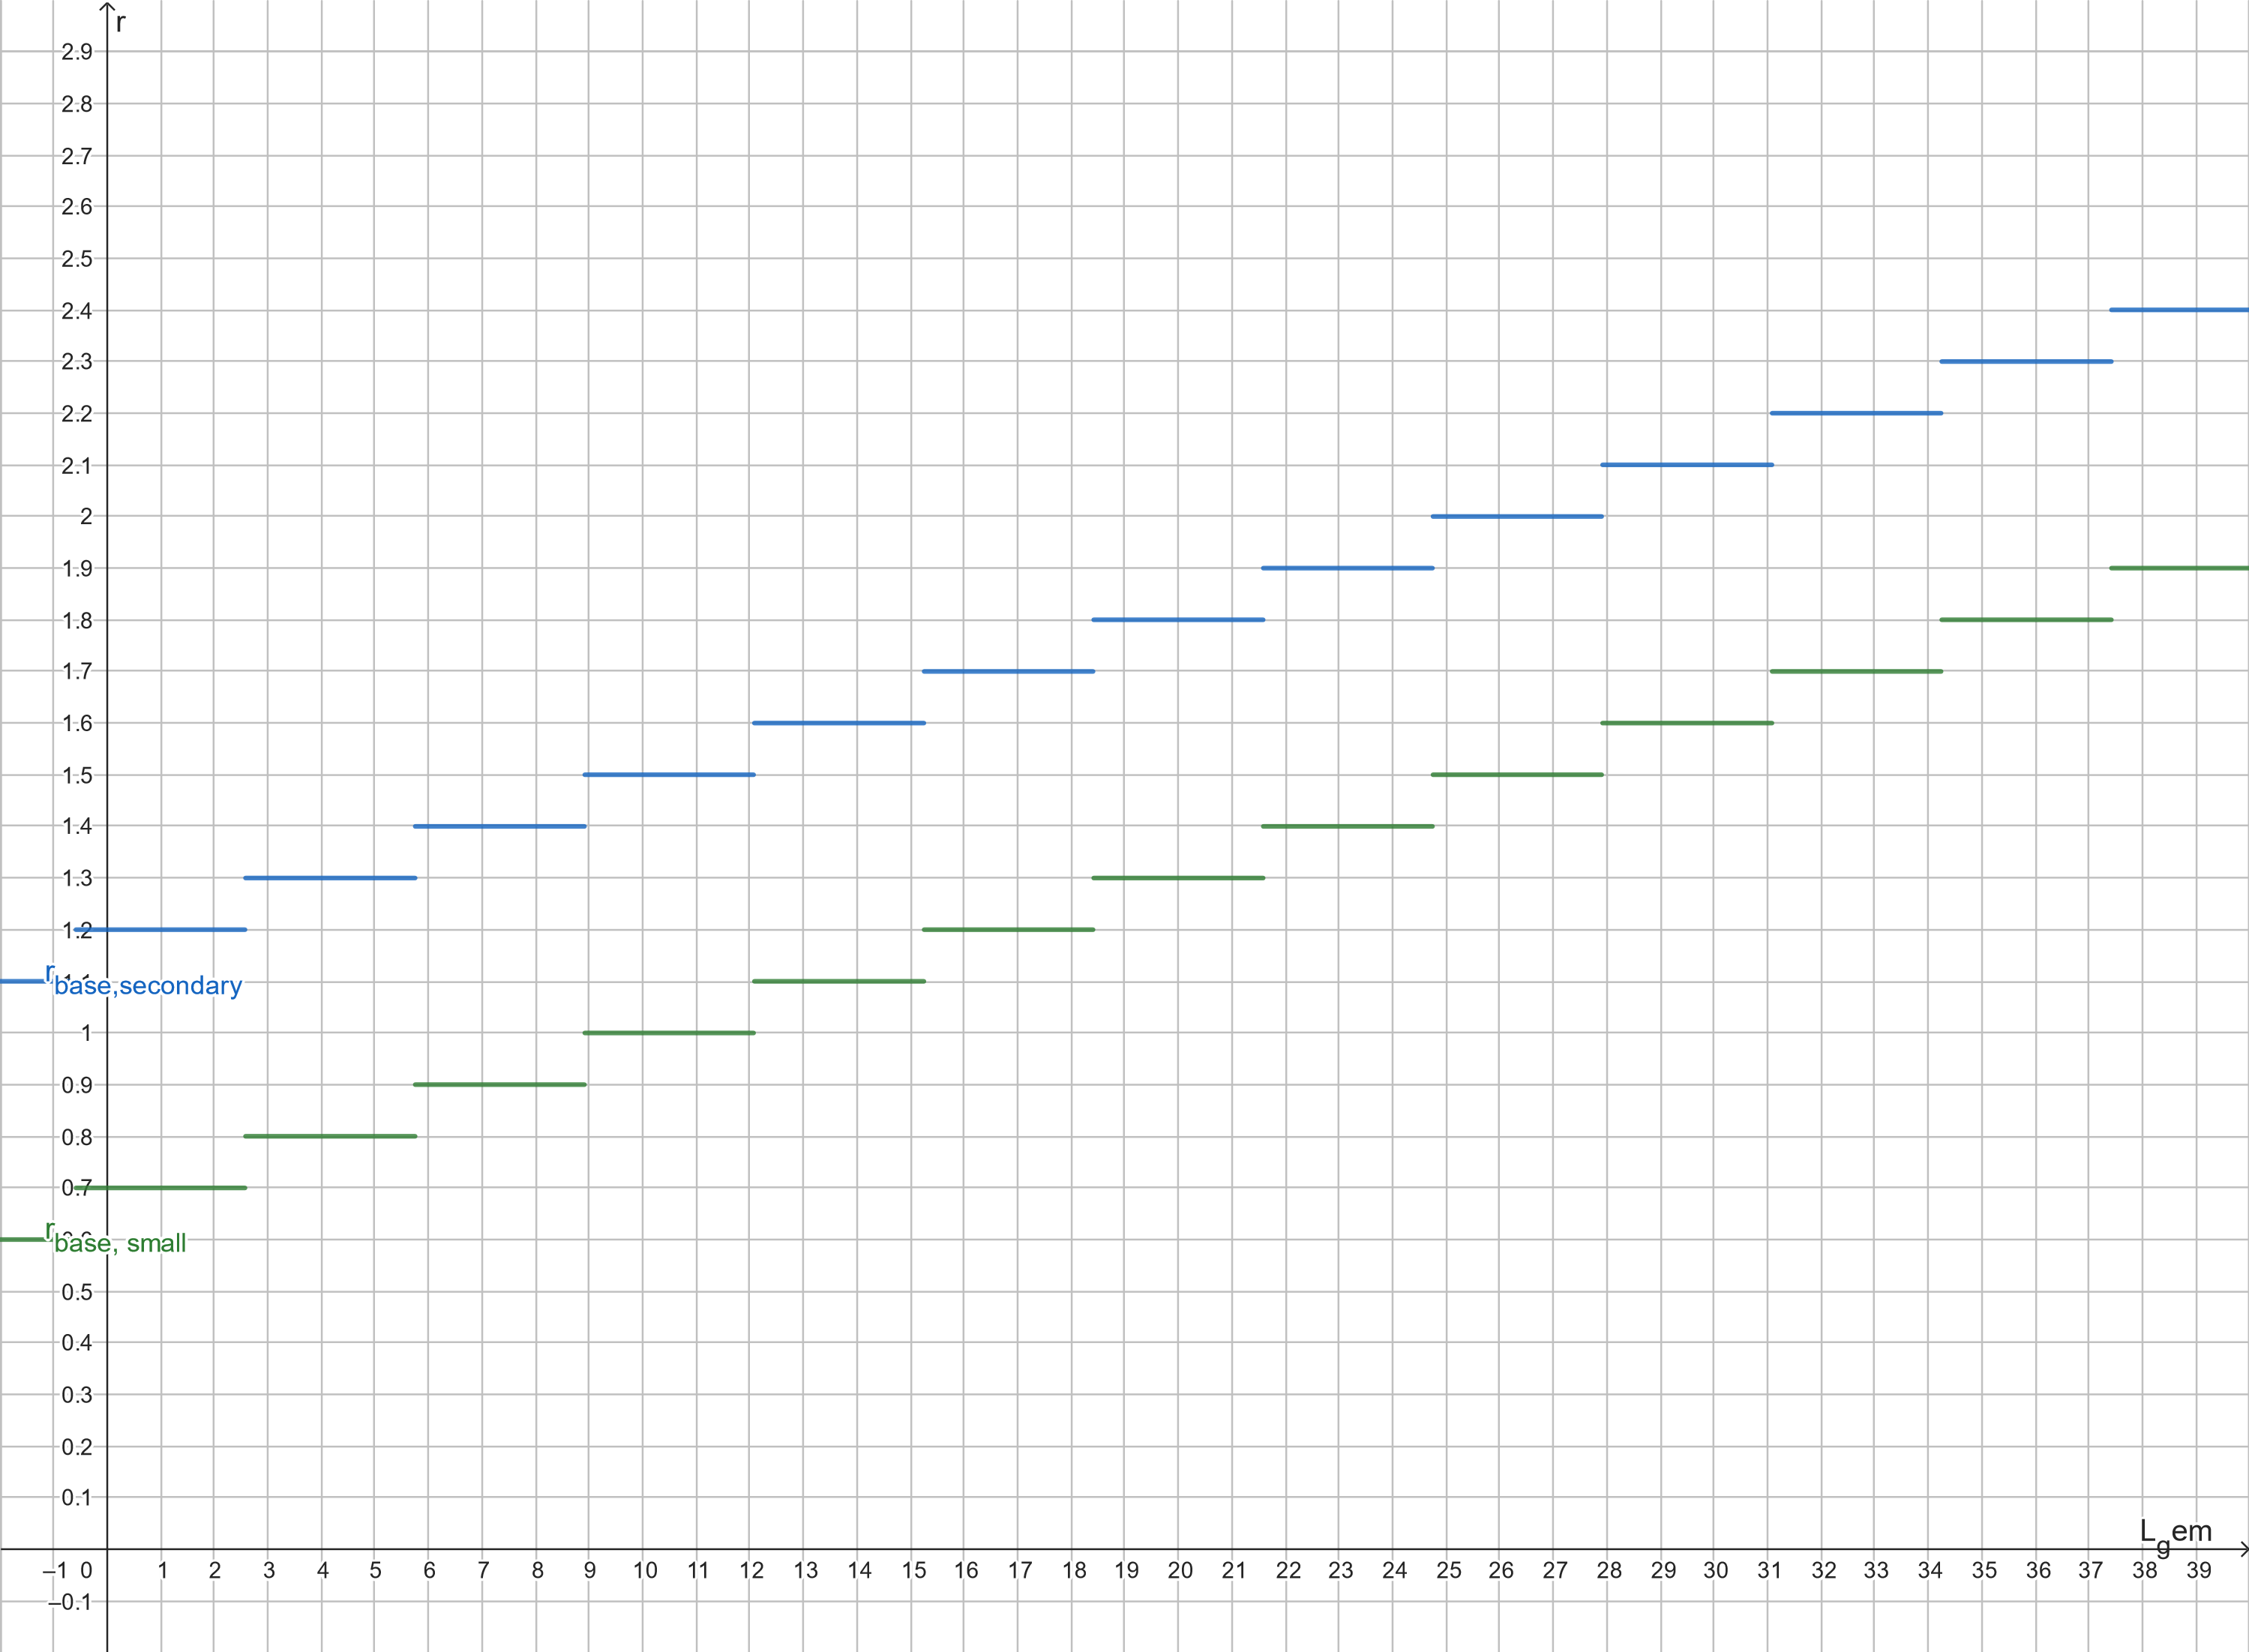
\includegraphics[width=\linewidth]{./02_Illustrations/Diagram_BaseRadToGemLevel.png}
	\caption{Diagram: base radius depending on gem level}
	\label{fig:Diagram_BaseRadToGemLevel}
\end{figure}

\begin{equation}
	X_\text{AoE} = 1 + \sum{\texttt{\# increased area of effect}}
\end{equation}

\begin{equation}
	r_\text{small} = \frac{r_\text{base, small}}{\sqrt{X_\text{AoE}}}
\end{equation}

\begin{equation}
	r_\text{secondary} = \frac{r_\text{base, secondary}}{\sqrt{X_\text{AoE}}}
\end{equation}


\begin{equation}
	p = \left(\frac{\frac{r_\text{base, small}}{\sqrt{X_\text{AoE}}} + r_\text{enemy} - \SI{0.1}{\meter}}{\frac{r_\text{base, secondary}}{\sqrt{X_\text{AoE}}}}\right)^2
\end{equation}

\subsection{Example}
\begin{equation}
	L_\text{gem} = 25
\end{equation}
\begin{equation}
	r_\text{base, small}(25) = \SI{1.5}{\meter}
\end{equation}
\begin{equation}
	r_\text{base, secondary}(25) = \SI{2}{\meter}
\end{equation}
\begin{equation}
	r_\text{enemy} = \SI{0.3}{\meter}
\end{equation}
\begin{align}
	p &= \left(\frac{\frac{\SI{1.5}{\meter}}{\sqrt{X_\text{AoE}}} + \SI{0.3}{\meter} - \SI{0.1}{\meter}}{\frac{\SI{2}{\meter}}{\sqrt{X_\text{AoE}}}}\right)^2\\
	&= \left(\frac{\frac{\SI{1.5}{\meter}}{\sqrt{X_\text{AoE}}} + \SI{0.2}{\meter}}{\frac{\SI{2}{\meter}}{\sqrt{X_\text{AoE}}}}\right)^2
\end{align}

\begin{figure}
	\centering
	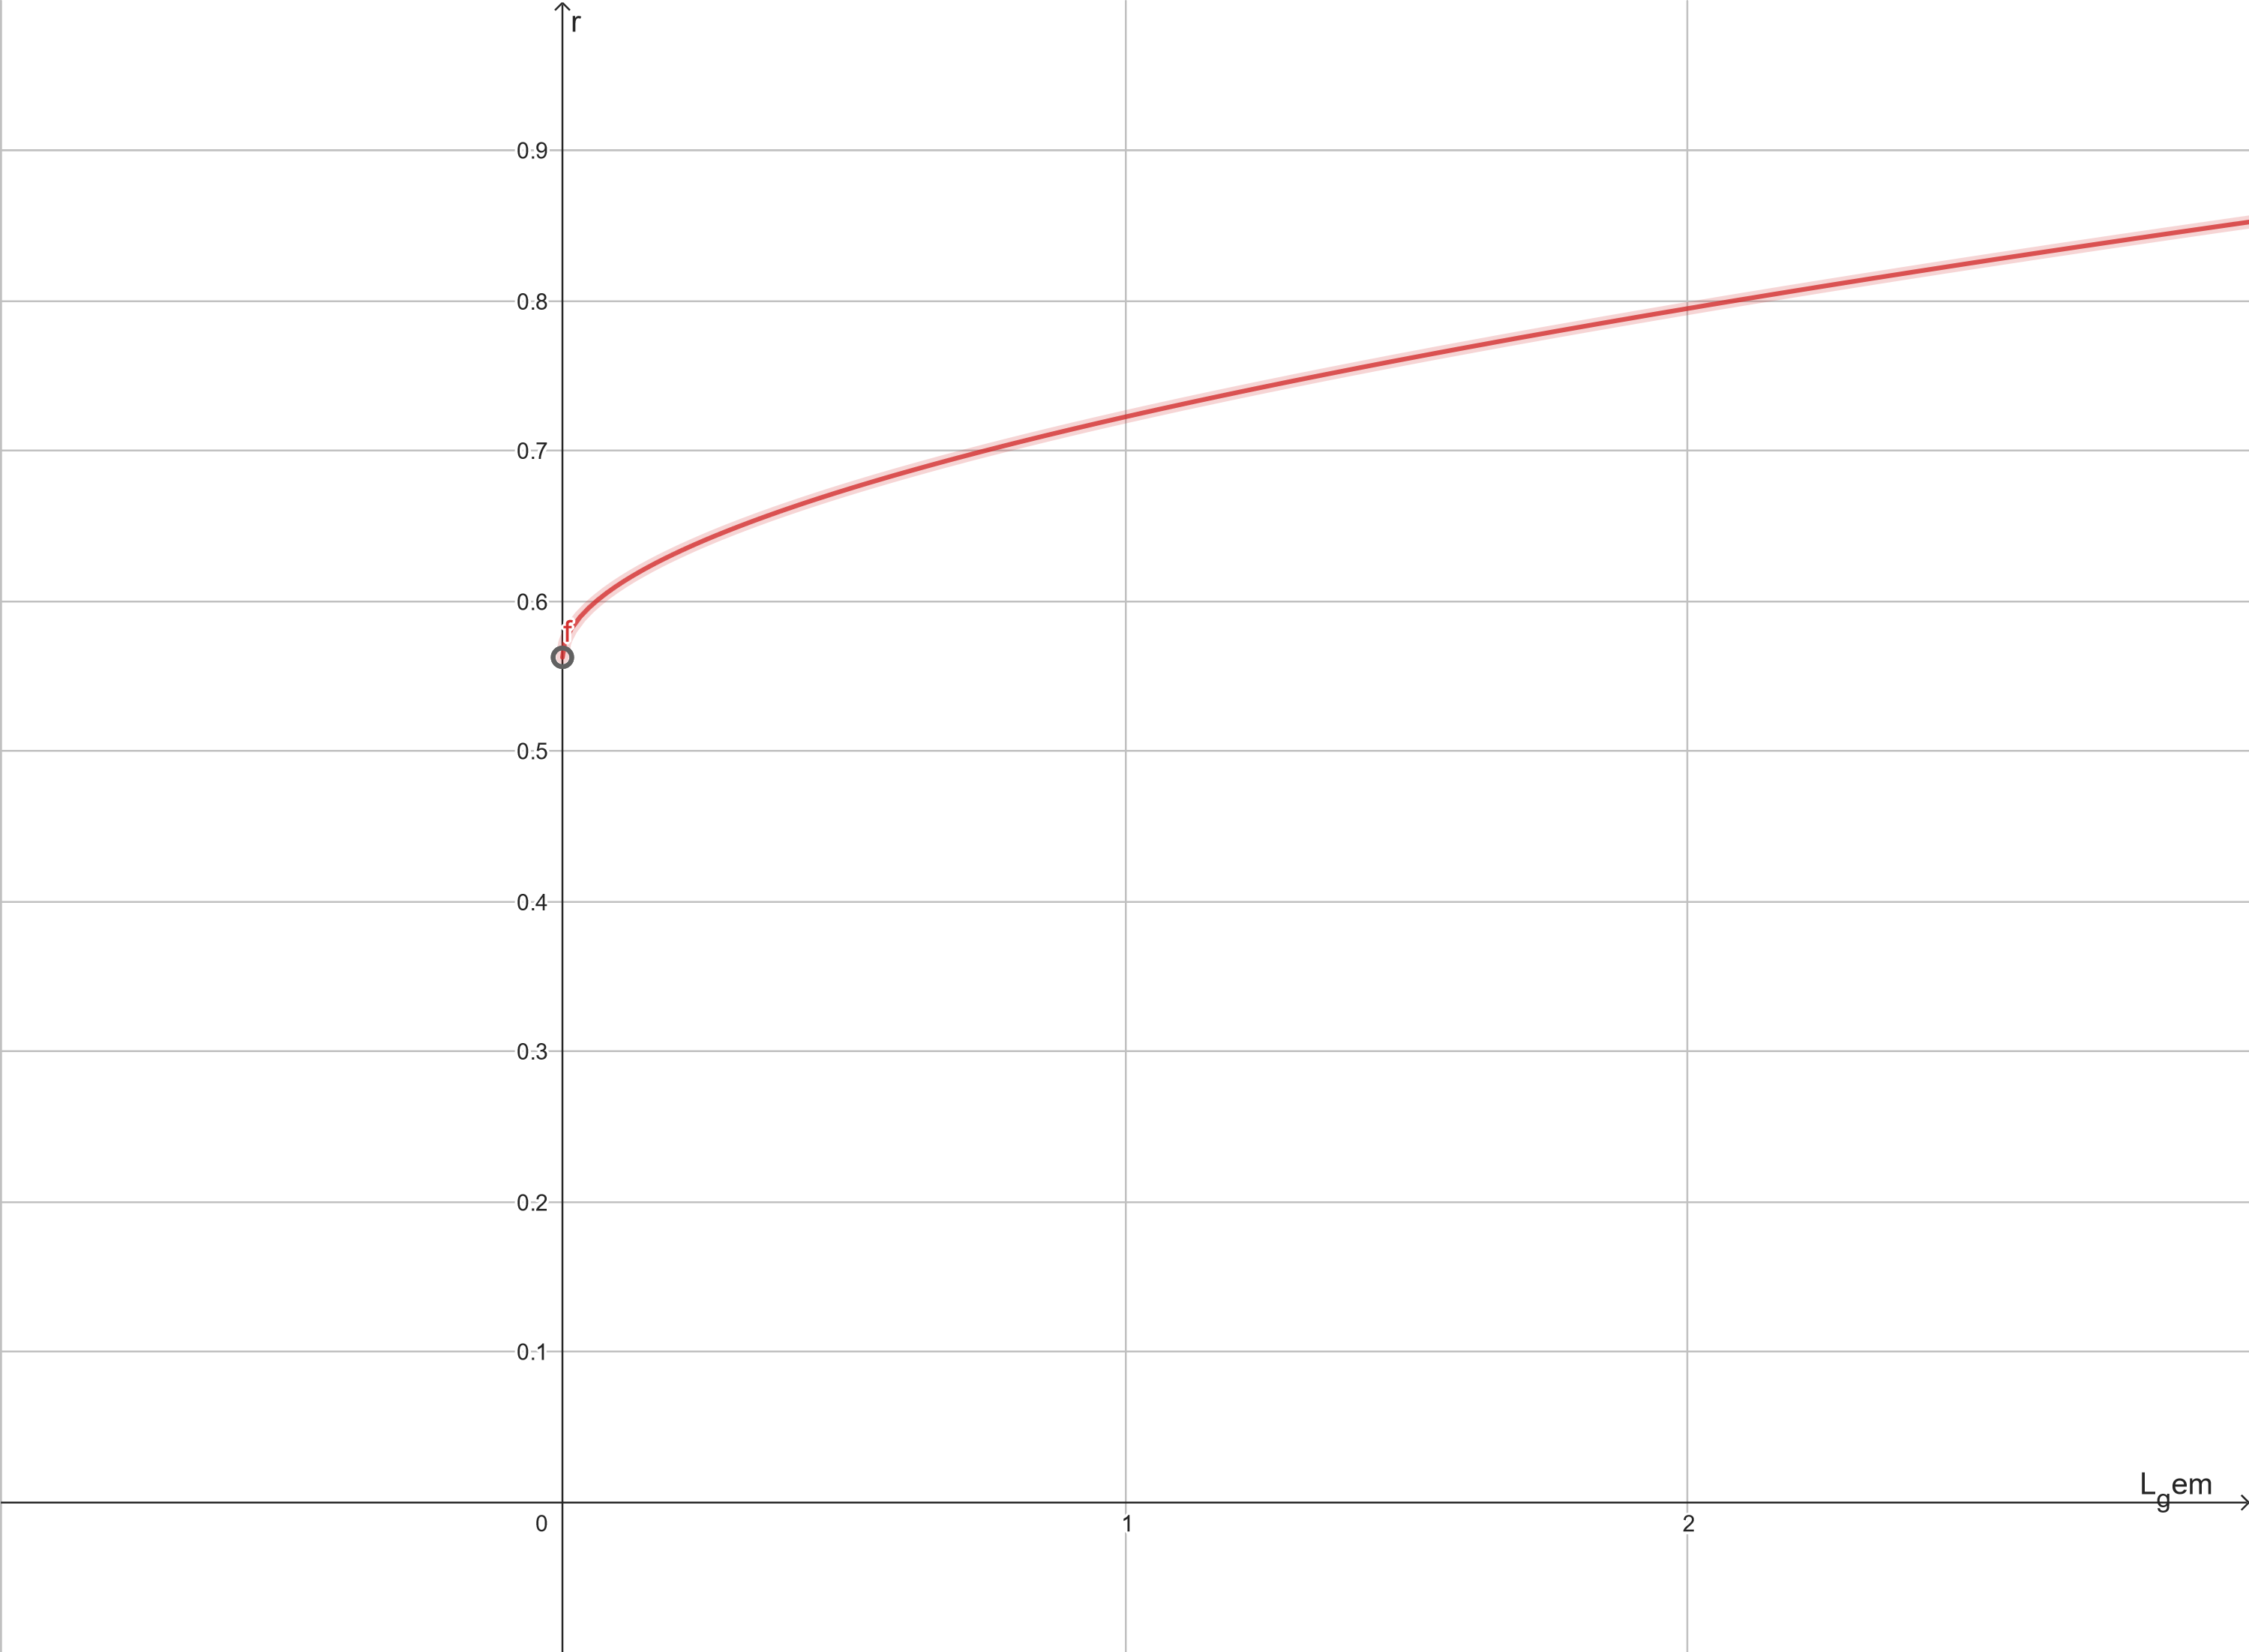
\includegraphics[width=\linewidth]{./02_Illustrations/Diagram_IncAoEToOverlappingChance_GLvL25.png}
	\caption{Diagram: overlapping chance depending on AoE-Multiplier with $L_\text{gem} = 25$}
	\label{fig:Diagram_IncAoEToOverlappingChance_GLvL25}
\end{figure}
